% THIS IS AN EXAMPLE DOCUMENT FOR VLDB 2012
% based on ACM SIGPROC-SP.TEX VERSION 2.7
% Modified by  Gerald Weber <gerald@cs.auckland.ac.nz>
% Removed the requirement to include *bbl file in here. (AhmetSacan, Sep2012)
% Fixed the equation on page 3 to prevent line overflow. (AhmetSacan, Sep2012)

\documentclass{vldb}
\usepackage{graphicx}
\usepackage{balance}  % for  \balance command ON LAST PAGE  (only there!)


\begin{document}

% ****************** TITLE ****************************************

\title{Data Integration On Multi-Cloud Environments}

% possible, but not really needed or used for PVLDB:
%\subtitle{[Extended Abstract]
%\titlenote{A full version of this paper is available as\textit{Author's Guide to Preparing ACM SIG Proceedings Using \LaTeX$2_\epsilon$\ and BibTeX} at \texttt{www.acm.org/eaddress.htm}}}

% ****************** AUTHORS **************************************

% You need the command \numberofauthors to handle the 'placement
% and alignment' of the authors beneath the title.
%
% For aesthetic reasons, we recommend 'three authors at a time'
% i.e. three 'name/affiliation blocks' be placed beneath the title.
%
% NOTE: You are NOT restricted in how many 'rows' of
% "name/affiliations" may appear. We just ask that you restrict
% the number of 'columns' to three.
%
% Because of the available 'opening page real-estate'
% we ask you to refrain from putting more than six authors
% (two rows with three columns) beneath the article title.
% More than six makes the first-page appear very cluttered indeed.
%
% Use the \alignauthor commands to handle the names
% and affiliations for an 'aesthetic maximum' of six authors.
% Add names, affiliations, addresses for
% the seventh etc. author(s) as the argument for the
% \additionalauthors command.
% These 'additional authors' will be output/set for you
% without further effort on your part as the last section in
% the body of your article BEFORE References or any Appendices.

\numberofauthors{5} %  in this sample file, there are a *total*
% of EIGHT authors. SIX appear on the 'first-page' (for formatting
% reasons) and the remaining two appear in the \additionalauthors section.

\author{
% You can go ahead and credit any number of authors here,
% e.g. one 'row of three' or two rows (consisting of one row of three
% and a second row of one, two or three).
%
% The command \alignauthor (no curly braces needed) should
% precede each author name, affiliation/snail-mail address and
% e-mail address. Additionally, tag each line of
% affiliation/address with \affaddr, and tag the
% e-mail address with \email.
%
% 1st. author
\alignauthor 
Daniel A. S. Carvalho\\
	   \affaddr{(Supervised by Chirine Ghedira-Guegan)}\\
       \affaddr{Universit\'e Jean Moulin Lyon 3}\\
       \affaddr{Centre de Recherche Magellan - IAE}\\
       \affaddr{Lyon, France}\\
       \email{daniel.carvalho@univ-lyon3.fr} 
}       
%% 2nd. author
%\alignauthor 
%Pl\'acido A. Souza Neto\\
%       \affaddr{Federal Institute of Rio Grande do Norte}\\
%       \affaddr{Natal, Brazil}\\
%       \email{first.last@ifrn.edu.br}
%% 3rd. author
%\alignauthor Chirine Ghedira-Guegan\\
%       \affaddr{Universit\'e Jean Moulin Lyon 3}\\
%       \affaddr{Centre de Recherche Magellan - IAE}\\
%       \affaddr{Lyon, France}\\
%       \email{first.last@univ-lyon3.fr}
%\and  % use '\and' if you need 'another row' of author names
%% 4th. author
%\alignauthor Nadia Bennani\\
%       \affaddr{LIRIS - INSA}\\
%       \affaddr{Lyon, France}\\
%       \email{first.last@insa-lyon.fr}
%% 5th. author
%\alignauthor Genoveva Vargas-Solar\\
%       \affaddr{CNRS-LIG}\\
%       \affaddr{Grenoble, France}
%       \email{first.last@imag.fr}
%}

% There's nothing stopping you putting the seventh, eighth, etc.
% author on the opening page (as the 'third row') but we ask,
% for aesthetic reasons that you place these 'additional authors'
% in the \additional authors block, viz.
%\date{30 July 1999}
% Just remember to make sure that the TOTAL number of authors
% is the number that will appear on the first page PLUS the
% number that will appear in the \additionalauthors section.

\additionalauthors{
  Additional authors: John Smith 
  (The Th{\o}rv\"{a}ld Group, {\texttt{jsmith@affiliation.org}}), 
  Julius P. Kumquat 
  (The \\Kumquat Consortium, 
  {\small \texttt{jpkumquat@consortium.net}}), and 
  Ahmet Sacan 
  (Drexel University, 
  {\small \texttt{ahmetdevel@gmail.com}}).}

\maketitle

\begin{abstract}
In the traditional databases theory, data integration is a problem of merging data from data sources in order to provide a unified view of this data to the user. This PhD project address data integration in multi-cloud environments. Current data integration systems implies consuming data from data services deployed in cloud contexts and integrating the results. The project takes a new angle of the problem by proposing an SLA-based approach, which given a user query and her integration preferences, to match the user preferences (such as whether she accepts to pay for the data, its provenance, freshness and how much she is ready to pay for the integration, among others) with the services' SLA while delivering the results. The objective is to enhance the quality on data integration taking into consideration the economic model imposed by the cloud. Our preliminary experiments have shown that quality can be enhanced and the cost of the integration results can be minimized by using our approach. 
\end{abstract}


\section{Introduction}
%Integrating data across different databases, and provide an unique view of it to the user, is a problem in the database domain (called data integration).
Data integration problem has been studied by many researchers in the database domain.
This can be seen in the service-oriented architecture as a service composition issue, such as given a query, the objective is to lookup for data services and compose them in order to achieve a desired result. 
%
%Finding the best service composition to answer a query can be computationally costly. 	
However, it is computationally costly to find the best service composition to answer a query. 
Furthermore, executing the composition can lead to retrieve and process data collections that can require important memory, storage and computing resources.
The on-demand resource provision imposed by the cloud computing architecture opens challenges to data processing and management.
%The cloud architecture allows and opens challenges to the data integration once such architecture give us an unlimited access to resources. 
%The possibility of having an unlimited access to resources, the resource management, the geographically distributed location of services, and the economic model imposed by the cloud architecture open challenges to data integration solutions.
Data integration has evolved with the emergence of data services that
deliver data under different quality conditions related to data freshness, cost, reliability,
availability, among others. Data are produced continuously and on demand in huge
quantities and sometimes with few associated meta-data, which makes the
integration process more challenging. Some approaches express data integration
as a service composition problem where given a query the objective is to lookup
and compose data services that can contribute to produce a result. Finding the
best service composition that can answer a query can be computationally costly.
Furthermore,  executing the composition can lead to retrieve and process data
collections that can require important memory, storage and computing resources.     

This problem has been addressed in the service-oriented
domain~\cite{Barhamgi2010,Benouaret2011,ba2014}.
Generally, these solutions deal with query rewriting problems.
\cite{Barhamgi2010} proposed a query rewriting approach which processes queries
on data provider services. \cite{Benouaret2011} introduced a service composition
framework to answer preference queries. In that approach, two algorithms based
on~\cite{Barhamgi2010} are presented to rank the best rewritings based on previously computed scores.
\cite{ba2014} presented an algorithm that produces and order rewritings
according to user preferences. Yet, to our knowledge few works consider quality
measures associated both to data services and to user preferences in order to
guide the rewriting process. 

Computing resources are delivered as services by the cloud. Services are billed and agreed between service providers and service customers under service level agreement (SLA) contracts.
Both sides must agree together on quality conditions and penalties under which the service is delivered. 
%Generally, those conditions and penalties associated to its violation are defined in service level agreement (SLA). 
Several researches have reported their studies on SLA in different domains~\cite{AlhamadDC11}.
SLA proposals for cloud computing could be divided in two groups: (i) works developing tools and methods to help on SLA negotiation and enforcement phase~\cite{rak2013,Mavrogeorgi2013}; and (ii) approaches that monitor contracts and cloud resources in order to detect and avoid SLA violations~\cite{Leitner2010,Maarouf2015}. To our knowledge, SLA publications have not been yet integrated to data integration in a multi-cloud environment.

Based on these concepts and open challenges, the goal of this work is to present
a data integration solution concerning a service-based query rewriting algorithm guided by SLA's.
Our work addresses these issues and proposes the algorithm (we
called \textit{Rhone}) with two original aspects: (i) the user can express her
quality preferences and associate them to her queries; and (ii)  service's quality aspects defined on Service Level Agreements (SLA) guide service selection and the whole rewriting process.
Yet, to the best of our knowledge, we have not identified any other work that uses SLA to guide the entire data integration solution.

This paper is organized as follows. Section ~\ref{sec:disla} discusses
about data integration and service level agreements (SLA).
Section~\ref{sec:scenario} contains the running scenario and challenges.
Section~\ref{sec:relatedwork} presents some related works.
Section~\ref{sec:rhone} describes the \textit{Rhone} algorithm and its
formalization.
Experiments and results are described in the section~\ref{sec:experiments}. 
Finally, section~\ref{sec:conclusion} concludes the paper and discusses future works.


\section{Related works}
Related works rely on four topics: 
(\textit{i}) data integration and data quality in the database domain;
(\textit{ii}) data integration approaches in the cloud and in service-oriented contexts; 
(\textit{iii}) query rewriting approaches; and 
(\textit{iv}) service level agreements for cloud computing.

Data integration has been widely discussed in the database domain.
\cite{Lenzerini:2002} discussed theoretical aspects in data integration including modeling applications, query evaluation, dealing with inconsistencies and reasoning queries.
Moreover, \cite{Halevy:2001} reviewed several query rewriting approaches. 
\cite{Batini2006} surveyed data quality aspects in data integration systems. 
\cite{Scannapieco:2004} presented a data quality broker that allows to submit queries with associated quality requirements over a global schema and to provide results according to them.

\cite{Correndo2010,ElSheikh2013} performed data integration in service-oriented contexts, particularly considering data services. However, they  consider computing resources consumption versus performance for guiding the data integration process. \cite{YauY08} addressed data privacy  to integrate data collected from different data services. \cite{Tian2010} proposed an inter-cloud data integration system considering privacy requirements and the cost for protecting and processing data. Even if \cite{Scannapieco:2004,Tian2010,YauY08} tackled quality aspects of the integration,  other crucial aspects  should be studied, for example data consumers requirements and constraints, data providers, the associated infrastructures and the data quality itself. It is also important to include these criteria in the way services are composed to produce  query plans.

As traditional databases theory, data integration on cloud and service-oriented context deals with query rewriting issues. Existing works like~\cite{ba2014,Barhamgi2010,Benouaret2011,Umberto} have refered it as a service composition problem. Given a query, the objective is to lookup and compose data services that can contribute to produce a result. In general, these works must address performance issues, because they use algorithms that can become expensive according to the complexity of the query and on the number of available services. Although \cite{ba2014,Benouaret2011} have considered preferences and scores to produce rewritings, the multi-cloud context introduces new requirements and constraints to the integration process. Currently, the approaches are not sufficient to cover the new challenges. Thus, they should be revisited and adapted in order to make the integration efficient in this new environment. 

Service level agreements (SLA) have been widely adopted in different domains to specify what service consumer can expect from the service delivered by a service provider. Research contributions in cloud computing concern (i) SLA management; (ii) inclusion of security requirements on SLAs; (iii) SLA negotiation; (iv) SLA matching; and (v) monitoring and allocation of cloud resources to detect and avoid SLA violations. 
%Research contributions in cloud computing mainly concern (i) SLA negotiation phase (step in which the contracts are established between customers and providers) and (ii) monitoring and allocation of cloud resources to detect and avoid SLA violations.
We strongly believe that SLAs can be used  to explicitely introduce the notion of quality in the current data integration solutions. In this sense, the use of SLAs to guide the entire data integration in a multi-cloud context seems original and promising for providing new perspectives to the data integration problem.


\section{Contributions}
Escrever um paragrafo resumindo as contribuicoes pretendidas no projeto e depois em subsecoes falar de alguns pontos principais... approach, model, schema, algoritmo... fazer essa imagem da abordagem no inkscape...

To explain our solution, in this section we present a metamodel that depicts implied entities and their relationship. 
Then a meta-process will introduce the functionalities of the proposed solution.
%To illustrate our problem, we proposed a metamodel to show relationship among the entities that are implied in our proposal (Figure~\ref{fig:scenario}).

According to our metamodel (Figure~\ref{fig:scenario}), the \textsl{Multi-Cloud} is configured as a set of \textsl{Cloud Infrastructures}. \textsl{Data producers} and \textsl{Data consumers} subscribe to \textsl{Cloud infrastructures}. 
Their subscription credentials are illustrated thanks to a \textsl{SLA} (\textsl{Consumer SLA} or \textsl{Producer SLA}) defining what the \textsl{Cloud infrastructure} offers to them through their subscription. 
\textsl{Data} are provided and consumed by \textsl{Data Producers} and \textsl{Data Consumers}, respectively. The \textsl{integration SLA} is a new type of SLA we introduce  to include the data regarding the entire integration process, user requirements and preferences, the \textsl{data producers} selected according to the constraints imposed by the environment, among others.

\begin{figure}[th!]
\center
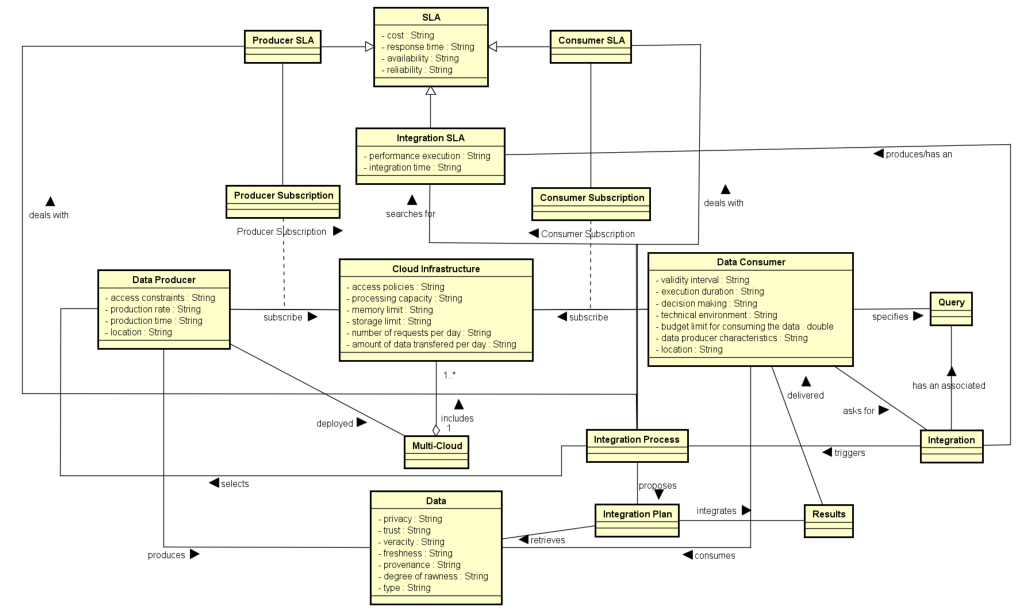
\includegraphics[scale=0.43]{metamodel.pdf}
\caption{Data integration metamodel}\label{fig:scenario}
\end{figure}

We propose a data integration meta-process (see Figure~\ref{fig:metaprocess}) consisting of three macro-steps (query management, SLA management and query rewriting) which take into account  the four  dimensions (\textsl{Data consumer}, \textsl{Data Producer}, \textsl{Cloud Infrastructures} and \textsl{Data}) described by the metamodel.
A meta-process workflow defines data integration process activities: \textit{first}, query management activities  to define the user query and preferences; \textit{second}, SLA management activities  to search and reuse previous SLAs used on integration (what we call \textsl{integration SLA}), and to create a new \textsl{integration SLA} for the current request; \textit{third}, query rewriting activities (as we partially described in~\cite{carvalho2016}) to search and filter \textsl{data producers}, to generate and execute the integration plan, and to compute results; \textit{finally}, other SLA management activities  to enforce the SLA associated to the involved services, and to update and store the final \textsl{integration SLA}. 

\begin{figure}[h!]
\center
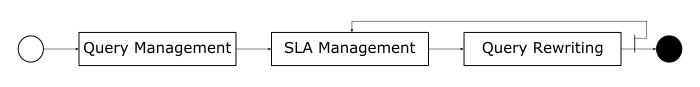
\includegraphics[scale=0.40]{meta-process.png}
\caption{Data integration meta-process}\label{fig:metaprocess}
\end{figure}

The activities defined in our meta-process bring the following challenges to our research:
\begin{enumerate}
\item \underline{SLA design}. The issue is what are the important information that should be inserted in the integration SLA to facilitate further integration? These information should be collected and stored during the integration to help next integrations.
\item \underline{Integration reuse}. How  to exploit cleverly the past integration processes? The new kind of SLA should be designed to include the information concerning the user requirements and preferences, the user query and the services used in the integration that satisfy the requirements, preferences and constraints imposed by the multi-cloud. Moreover, we must identify important information collected during the integration that should be saved  to be reused in the next integration making the entire process more efficient. 
%\item \underline{Query rewriting activities}. The query rewriting activities deal with a complex matching process of user requirement and preferences with constraints imposed by the context, and expressed in different SLAs. Furthermore, during the execution, it is also necessary to enforce the SLAs associated to the \textsl{data producers}. In this process, perhaps a given \textsl{producer} can run out of resources for processing the request.
\item \underline{Rewriting process}. How to optimize it to make the execution time acceptable? Retrieving, integrating and delivering are tasks that requires a large amount of resources and processing time. Thus, it is necessary to study a clever manner to make efficient the overall execution, and also there is an important decision making step while choosing the best cloud to proceed with the integration.
\end{enumerate}

%Taking into consideration at real-time the entities presented in our metamodel and our meta-process, we propose a SLA-based data integration process adapted to the multi-cloud below.
%%
%A users specifies a query according to his/her needs and requirements. In addition, he/she defines a set of preferences and associate them to the query. Given a query and user preferences, previous integration SLAs (that are associated to a previous integration) that matches with the actual query and preferences are searched. If a match is found, the information about this previous integration is reused and a new integration SLA is created using this information. On the other hand, if no match is found, a new integration SLA is created without any previous information. Then, a set of query rewriting activities are performed to generate the execution plan. Results are computed and the integration SLA is updated and stored to be used in a next integration request. The query rewriting activities sub-process include (i) searching for data producers that can produce an answer to the query;  (ii) filtering data producers according to the user preferences, to the consumer SLAs and to the producer SLAs. This means it is necessary to verify if the data producer is out of resources or not, and if the consumer has enough resources to process the data provided by the producer; (iii) generating the execution plan according to the SLAs; (iv) enforcing the SLAs associated to the involved services; and (v) executing the integration plan. Computing results sub-process retrieves data, integrates results and deliver them.
%

%\textsc{\begin{figure}[h!]
%\center
%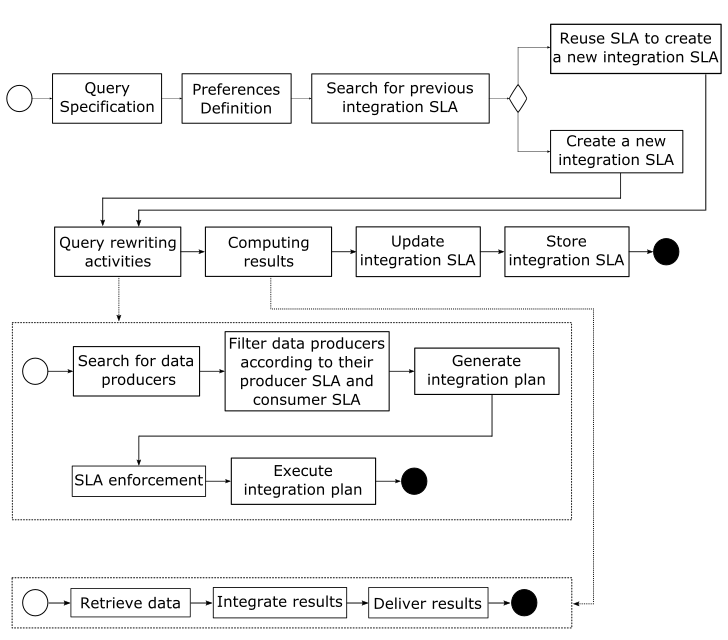
\includegraphics[scale=0.50]{process.png}
%\caption{Data integration process}\label{fig:process}
%\end{figure}}


%Given a user \textit{query}, a set of associated user \textit{preferences} and \textsl{Data Consumers}:
%\\
%\textbf{\underline{SLA derivation}}. In this step, we compute what we call an \textsl{integration SLA} that matches user' integration requirements (including quality constraints and data requirements) with the \textsl{SLA}'s provided by \textsl{data producers}, given a specific user cloud subscription. The user may have general requirements depending on the context he/she wants to integrate his/her data such as economic cost, bandwidth limit, free services, and storage and processing limits. The \textit{SLA derivation} is the big challenge while dealing with SLAs and particularly for adding quality dimensions to data integration. Furthermore, the \textsl{integration SLA} guides the query evaluation, and the way results are computed and delivered. \\
%\textbf{\underline{Filtering data services}}. The \textsl{integration SLA} is used (i)
%to filter previous \textsl{integration SLA} derived for a similar request in order to reuse results; or (ii) to filter possible \textsl{data producers} that can be used for answering the query. \\ %The SLA exported by a selected \textit{cloud service} should satisfy the user \textit{preferences}. \\
%\textbf{\underline{Query rewriting}}. Given a set of \textit{data producers} that can
%potentially provide data for integrating the query result, a set of service compositions is generated according to the \textsl{integration SLA} and the agreed \textsl{Producer SLA} of each \textsl{data producer}. \\
%\textbf{\underline{Integrating a query result}}. The service compositions are
%executed with services from one or several clouds where the user has a
%subscription.
%The execution cost of service compositions must fulfill the \textsl{integration
%SLA}. The clouds resources needed by the user to execute the composition and how
%to use them is decided taking in consideration the economic cost determined by
%the data to be transferred, the number of external calls to services, data storage and delivery cost.

%The algorithm 1 describes in general lines our approach which integrate data
%from multi-cloud environments considering quality aspects.
%%
%As input, we consider (1) a user query $Q$; (2) a set of user preferences $P$;
%(3) a user cloud subscription $C$; (4) a set of previous \textit{integrated SLA}
%$\bigSLA$, obtained from a local register; (5) a set of \textit{data services}
%$DS$; (6) a set of \textit{data processing services} $DPS$; and (7) a set of \textit{cloud providers} $CP$. As output, the integration results $IR$ is delivered to the user while fulfilling her preferences and cloud subscription.
%%
 
%The approach begins looking for previous \textit{integrated SLAs} in our
%local registry. From each \textit{integrated SLA} we verify if it matches
%the user' query and preferences (lines 2 - 6), and adding them to the set $pI$ (line 4).
%%
%If previous \textit{integrated SLA} matches (line 7), the one that
%partially matches with the user preferences is selected (line 8).
%%
%Then, a new \textit{integrated SLA} is computed for user query based on the
%previous \textit{integrated SLA}, her preferences and cloud subscription (line 9).
%%
%The service compositions produced to a previous query is reused based its \textit{integrated SLA} ($sI$). 
%%
%Otherwise, a new \textit{integrated SLA} is created to user request given the query, her preferences and cloud subscription (line 11). 
%%
%The SLA information of $\mathit{DS}$ and $\mathit{DPS}$ is extracted and included in the set of \bigS (line 12). 
%%
%This new \textit{integrated SLA} is updated by calling the \textit{Rhone} procedure (line 13). 
%%
%The \textit{Rhone} is responsible of (i) selecting \textit{data services} (in $DS$) and \textit{data processing services} (in $DPS$) which satisfy the user preferences based on their SLAs; and (ii) producing service compositions that completely match with the query and fulfill the user preferences. 
%%
%Finally, the integration results ($IR$) are produced and delivered to the user considering her cloud subscription. 
%%
%Note that while executing compositions, it is necessary to satisfy the user requirements and cloud subscription, and also to dynamically update the \textit{integrated SLA} adding the information of contracts that were established to allow the integration. 
%%
%Finally, the \textit{integrated SLA} is stored in our registry to be used in a next query.   
%
%\begin{algorithm} 
%%\small
%\caption{ - SLA-based data integration}
%\label{qualityBasedAlgorithm}
%\begin{algorithmic}[1]
%\REQUIRE Query ($Q$), user preferences ($P$), user cloud subscriptions ($C$), a
%set of \textit{data services} ($\mathit{DS}$) and \textit{data processing services} ($\mathit{DPS}$) and a set of previous \textit{integrated SLA} ($\bigSLA$).
%\ENSURE Integration results delivered considering the user cloud subscription.
%%\STATE \textbf{function} $\mathit{SelectCandidateServices} (Q, \bigS)$
%%\STATE let $\bigSLA$ be a set of previous integrated SLA
%\STATE $pI \leftarrow \emptyset$
%\FORALL  {$SLA_{i}$ in $\bigSLA$}
%	\IF {$\mathit{macthes(Q, P, SLA_{i})}$}
%		\STATE $pI \leftarrow pI \cup \lbrace SLA_{i} \rbrace$		
%%		\FORALL  {$A_{j}$ in $S_{i}$}
%%			\IF {$Q.\mathit{notContains(A_{i})}$}
%%				\STATE $b \leftarrow \mathit{false}$	
%%				\STATE $\mathit{break}$
%%			\ENDIF
%%		\ENDFOR
%%		\IF {$b = true$}
%%			\STATE $\bigLS \leftarrow \bigLS \cup \lbrace S_{i} \rbrace$	
%%		\ENDIF
%	\ENDIF
%\ENDFOR
%\IF {$pI \neq \emptyset$}
%	\STATE $sI \leftarrow chooseBest(P, pI)$
%	\STATE $newSLA_{i} \leftarrow deriveSLA(sI, P, C)$
%%	\FORALL  {$SLA_{i}$ in $pI$}
%%		\STATE $sI \leftarrow choose(P,)$
%%	\ENDFOR
%\ELSE
%	\STATE $newSLA_{i} \leftarrow deriveSLA(Q, P, C)$
%	\STATE $\bigS \leftarrow extract(\mathit{DS}, \mathit{DPS})$
%	\STATE $newSLA_{i} \leftarrow updateSLA(Rhone(Q, \bigS))$
%\ENDIF
%\STATE $IR \leftarrow execute(newSLA_{i})$
%\STATE \textbf{return} $IR$
%\STATE \textbf{end function}
%\end{algorithmic}
%\end{algorithm} 

%\subsection{SLA-based query rewriting algorithm}
%To serve a proof of concept to our approach, we develop a query
%rewriting algorithm which is guided by users' integration requirements and
%service level agreements exported by different data services and cloud
%providers. Researches have refered to data integration as a service composition problem
%in which given a query the objective is to lookup and compose data services that
%can contribute to produce a result. Currently, we have formalized and developed a rewriting
%algorithm that considers user preferences and services' quality aspects while
%selecting services and producing rewritings called \textit{Rhone} (See algorithm
%\ref{algo-rhone}, invoked in the algorithm 1, line 12).
%The \textit{Rhone} algorithm consists in four macro steps: 
%\\
%\textbf{\underline{Selecting data services}}. The \textit{Rhone} looks for
%\textit{data services} (line 2) that can contribute to answer the query while
%satisfying the user' preferences; \\
%\textbf{\underline{Building candidate service descriptions}}. A candidate
%service description (CSD) describes how a \textit{data service} can contribute to answer the query. CSD maps a \textit{data service} (including its variables) to the entire query or part of it. For all selected services, the \textit{Rhone} tries to build CSDs when the mapping of variables is possible (line
%3). \\
%\textbf{\underline{Combining CSDs}}. All CSDs are combined (line 4) producing a
%list of CSD combinations. Each combination can be a rewriting of the query. \\
%\textbf{\underline{Producing rewritings}}. Each list of CSDs is checked in order
%to verify whether it is a rewriting of the query or not (line 9). To be a
%valid rewriting, it is forbidden to have CSDs covering the same part of the query.
%Rewritings are produced while the user' requirements are being respected (lines 6-14).
%%
%The originality of our algorithm concerns the functions ~\!\tqI{}, ~\!\tqT{} and ~\!\tqS{}.     
%They are responsible to initialize, check and increment user preferences
%associated to some aggregation like user constraints (total cost). This means
%that these preferences are initialized (line 6), and for each element in the CSD list they are incremented (line 11), and rewritings are produced while they are respected (line 8).  The result of this step is the list of valid rewritings of the query (line 14).
%
%\begin{algorithm}[h!]
%\small
%\caption{ - \textit{Rhone}}
%\label{algo-rhone}
%\begin{algorithmic}[1]
%\REQUIRE A query $Q$, a set of user preferences, and a set of concrete services $\bigS$.
%\ENSURE A set of rewritings $R$ that matches with the query and fulfill the user preferences.
%\STATE \textbf{function} $\mathit{Rhone} (Q, \bigS)$
% \STATE  $\bigLS \leftarrow \mathit{SelectCandidateServices}(Q, \bigS)$ \label{rhone:buildPCD}
% \STATE  $\bigLCSD \leftarrow CreateCSDs(Q, \bigLS)$
% \STATE  $I \leftarrow CombineCSDs(\bigLCSD)$
% \STATE $R\leftarrow \emptyset$
% \STATE ~\!\tqI{\agg{Q}} 
%    \STATE $p \leftarrow I.next()$
%    \WHILE {$p\ \neq\ \emptyset$ \AND ~\!\tqT{\agg{Q}}} 
%      \IF {\textit{isRewriting}$(Q, p)$}
%  \STATE $R\leftarrow R\,\cup \mathit{Rewriting}(p)$
%  \STATE ~\!\tqS{\agg{Q}}
%   \ENDIF
%      \STATE $p \leftarrow I.\mathit{next}()$
% \ENDWHILE
%    \STATE \textbf{return} $R$
%\STATE \textbf{end function}
%\end{algorithmic}
%\end{algorithm}
%
%To serve as a proof of concept to our approach, we intend to develop a query
%rewriting algorithm which is guided by users' integration requirements and
%service level agreements exported by different data services and cloud
%providers. The query rewriting is an important issue in data integration. In
%cloud computing, researches have refereed to it as a service composition problem
%in which given a query the objective is to lookup and compose data services that
%can contribute to produce a result. \cite{Barhamgi2010} proposed a query
%rewriting approach which processes queries on data provider services.
%\cite{Benouaret2011} introduced a service composition framework to answer
%preference queries. Two algorithms inspired on~\cite{Barhamgi2010} are presented
%to rank the best rewritings based on previously computed scores. \cite{ba2014}
%extended \cite{Umberto} and presented an refinement algorithm that produces and
%order rewritings according to user preferences and scores. In general, these
%works share the same performance problem depending on the size of the query and
%on the number of available services. Furthermore, they do not take into
%consideration user's integration requirements what can lead to produce
%rewritings that are not satisfactory to the user in terms of quality
%requirements and cost. Currently, we have formalized and developed a rewriting
%algorithm that considers user preferences and services' quality aspects while
%selecting services and producing rewritings called \textit{Rhone} (Invoked in the algorithm 1, line 12).                     
\begin{figure}[h!]
\centering
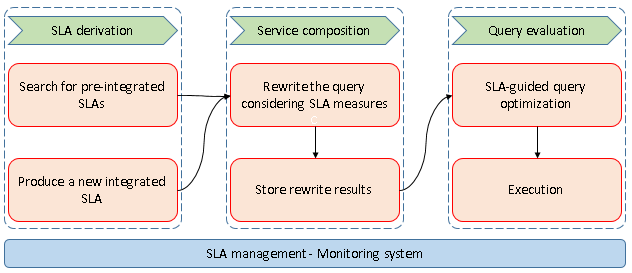
\includegraphics[scale=0.5]{general_approach}
\caption{A sample black and white graphic (.pdf format).}
\label{fig:generalapproach}
\end{figure}

\section{Preliminary results}
colocar parte dos resultados do adbis + um grafico do custo da reescrita..
We have developed a prototype of our query rewriting algorithm which takes into consideration users' requirements and services' quality aspects extracted from SLAs called \textsl{Rhone}.

Currently, our approach runs in a local controlled environment simulating a single-cloud including a service registry of 100 concrete services. Experiments were produced to analyze the algorithm's behavior concerning performance, and quality and cost of the integration. The figures~\ref{fig01} and \ref{fig02} summarize our first results.

\begin{figure}
\centering
\begin{subfigure}{.5\textwidth}
  \centering
  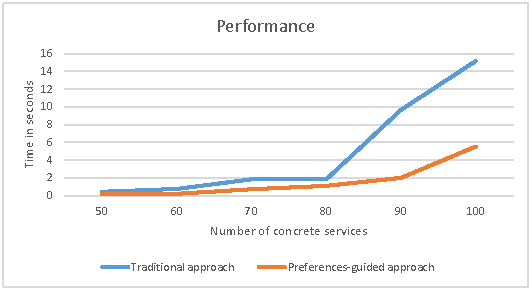
\includegraphics[scale=0.61]{fig1.pdf}
  \caption{Performance evaluation.}
  \label{fig01}
\end{subfigure}%
\begin{subfigure}{.5\textwidth}
  \centering
  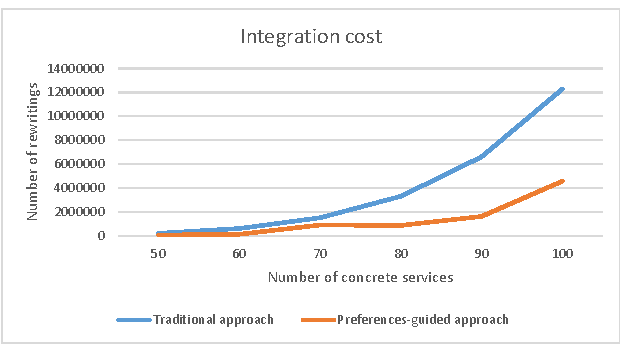
\includegraphics[scale=0.53]{fig2.pdf}
  \caption{Integration cost.}\label{fig02}
\end{subfigure}
\caption{\textit{Rhone} execution evaluation.}
\label{fig:figs-exp}
\end{figure}


%\begin{figure}[!h]
%\centering
%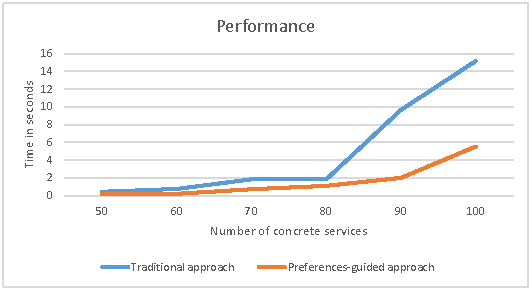
\includegraphics[scale=0.8]{fig1.pdf}
%\caption{Performance evaluation.}\label{fig01}
%\end{figure} 

The experiments include two different approaches: (i) the \textit{traditional approach} in which user preferences and SLAs are not considered; and (ii) the \textit{preference-guided approach} (P-GA) which considers the users' integration requirements and SLAs.
%
%\begin{figure}[!h]
%\centering
%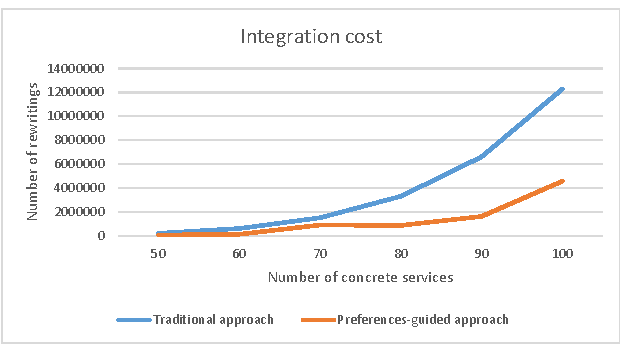
\includegraphics[scale=0.72]{fig2.pdf}
%\caption{Performance evaluation.}\label{fig02}
%\end{figure} 

The results P-GA are promisingly.  
The \textit{Rhone} increases performance reducing rewriting number which allows to go straightforward to the rewriting solutions that are satisfactory avoiding any further backtrack and thus reducing successful integration time (Figure~\ref{fig01}). Moreover, using the P-GA to meet the user preferences, the quality of the rewritings produced has been enhanced and the integration economic cost has considerable reduced while delivering the expected results (Figure~\ref{fig02}). However, the \textit{Rhone} still need to be tested in a large scale case and in a context of parallel multi-tenant to test efficacy.

\section{Conclusions}
recapitular as ideias do projeto e o que vamos fazer...
This work proposes a query rewriting algorithm for data integration quality
named \textit{Rhone}. Given a query, user preferences and a list of concrete services as input,
the algorithm derives rewritings in terms of concrete services that matches with the query and
fulfill the user preferences. The formalization and experiments are presented. The results 
show that the \textit{Rhone} reduces the rewriting number and processing time while considering 
user preferences and services' quality aspects extracted from SLAs to guide the service selection and rewriting.
We are currently performing improvements in the implementation and setting up a
multi-cloud simulation in in order to evaluate the performance of the
\textit{Rhone} in such context.  
% \end{document}  % This is where a 'short' article might terminate

% ensure same length columns on last page (might need two sub-sequent latex runs)

%ACKNOWLEDGMENTS are optional
%\section{Acknowledgments}
%ACKNOWLEDGMENTS are optional...

% The following two commands are all you need in the
% initial runs of your .tex file to
% produce the bibliography for the citations in your paper.
\bibliographystyle{abbrv}

\bibliography{vldb_sample}  
% vldb_sample.bib is the name of the Bibliography in this case
% You must have a proper ".bib" file
%  and remember to run:
% latex bibtex latex latex
% to resolve all references

\end{document}
